\documentclass[a4paper,anonymous,USenglish]{lipics-v2019}
\usepackage[utf8]{inputenc}
\usepackage{algorithm}
\usepackage{algpseudocode} % for pseudocode
\usepackage{tikz} % for figures
\usepackage{subcaption} % for subfigures

\title{Byzantine Eventual Consistency}

\author{Martin Kleppmann}{University of Cambridge}{mk428@cst.cam.ac.uk}{https://orcid.org/0000-0001-7252-6958}{Supported by a Leverhulme Trust Early Career Fellowship and by the Isaac Newton Trust.}

\author{Heidi Howard}{University of Cambridge}{hh360@cst.cam.ac.uk}{https://orcid.org/0000-0001-5256-7664}{}

\authorrunning{M. Kleppmann and H. Howard}
\Copyright{Martin Kleppmann and Heidi Howard}

\begin{CCSXML}
<ccs2012>
   <concept>
       <concept_id>10003752.10003809.10010172</concept_id>
       <concept_desc>Theory of computation~Distributed algorithms</concept_desc>
       <concept_significance>500</concept_significance>
       </concept>
   <concept>
       <concept_id>10002951.10003152.10003166.10003172</concept_id>
       <concept_desc>Information systems~Remote replication</concept_desc>
       <concept_significance>300</concept_significance>
       </concept>
 </ccs2012>
\end{CCSXML}

\ccsdesc[500]{Theory of computation~Distributed algorithms}
\ccsdesc[300]{Information systems~Remote replication}

\keywords{replication, Byzantine fault tolerance, eventual consistency}

\begin{document}
\maketitle
\begin{abstract}
    Byzantine agreement guarantees consistency provided that less than $1/3$ of processes are faulty.
    However, if more faults occur, we can still guarantee weaker consistency models. 
    In this paper we define one such model, which we refer to as Byzantine Eventual Consistency (BEC).
    We also introduce an algorithm that implements this consistency model, even in a system with arbitrarily many Byzantine-faulty processes, and prove that it ensures BEC.
\end{abstract}
\maketitle

\section{Introduction}

Byzantine agreement assumes that at most $f$ out of $n$ processes are Byzantine-faulty.
It is well established that without synchrony, Byzantine agreement is impossible if $n\leq3f$~\cite{Dwork:1988,Lamport:1982}.
If more than $f$ processes are faulty, neither safety (agreement) nor liveness can be guaranteed.
This is a problem because the assumption that no more than $f$ processes are faulty is not always a realistic threat model.

Byzantine failures are not necessarily independent: if an adversary can compromise one of the processes (e.g. due to a software vulnerability), it is likely that they can compromise a majority of processes, since they are likely to all be running the same software. 
Similarly, non-malicious software bugs are likely to affect many of the processes at once.
This issue was acknowledged in the pBFT paper, which states that: ``{\dots}each node should run different implementations of the service code and operating system{\dots}''~\cite{Castro:1999}~--- an assumption that is unrealistic for any system with more than a few processes, and is seldom true in practice today.
In some systems, such as open peer-to-peer networks that anybody can join, an adversary can spawn a large number of processes, and thus create a majority of Byzantine-faulty processes (this is known as a Sybil attack~\cite{Douceur:2002}).

This state of affairs raises the question: if Byzantine agreement cannot be achieved in the face of arbitrary numbers of Byzantine-faulty processes, what consistency model \emph{can} we achieve under that assumption?

In this paper we propose \emph{Byzantine Eventual Consistency} (BEC), a novel consistency model that can be achieved regardless of the number of Byzantine-faulty processes.
We define BEC in \S~\ref{sec:properties}, and in \S~\ref{sec:algorithm} we introduce an algorithm that achieves BEC (as proved in \S~\ref{sec:proof}).
In BEC, each process is a replica of some shared state, and any two correct replicas converge towards the same state as they communicate, even if they also communicate with arbitrarily many Byzantine-faulty processes.
Essentially, the algorithm ensures that faulty replicas cannot corrupt the state of correct replicas.

\section{Defining Byzantine Eventual Consistency}\label{sec:properties}

Algorithms for Byzantine agreement (or consensus) are often used to create an append-only log of values for state machine replication~\cite{Schneider:1990} (SMR), such as a blockchain~\cite{Bano:2019}.
The primary correctness criterion for such a log is that all correct processes observe the same sequence of values, even in the presence of up to $f$ Byzantine-faulty processes.
If we use these values as inputs to a deterministic state machine, that state machine goes through the same sequence of state transitions on each process, resulting in consistent replicas of the state.

This notion of creating an append-only log is typically formalised by requiring that for all executions of the consensus algorithm, the following properties hold:

\begin{description}
\item[Validity:] Any value decided by a correct process must have been proposed by one of the processes.
\item[Agreement:] If two correct processes decide a value for a certain position in the log, those values are the same.
\item[Liveness:] For any value proposed by one of the processes, all correct processes will eventually decide that value for some position in the log.
\end{description}

The agreement and liveness properties of Byzantine agreement assume that no more than $f$ processes are Byzantine-faulty, while liveness also assumes partial synchrony~\cite{Dwork:1988}.

We define Byzantine Eventual Consistency (BEC) using properties analogous to those of Byzantine agreement.
Rather than maintaining an append-only log, we assume that each process locally maintains a monotonically growing set of updates $\mathcal{U}$.
We then say that an algorithm ensures BEC if, for all executions of that algorithm, the following properties hold:

\begin{description}
\item[Validity:] Any update in the set of updates $\mathcal{U}$ of a correct process must have been proposed by one of the processes.
\item[Convergence:] When any two correct processes have both completed reconciliation, their sets of updates are the same. (The notion of ``completing reconciliation'' is defined below.)
\item[Liveness:] For any update proposed by one of the processes, that update will eventually be contained in the set of updates for all correct processes.
\end{description}

Like in Byzantine agreement, liveness in BEC requires a further assumption: namely, we assume that any network partitions are of a finite duration, i.e.\ that any two processes will eventually be able to exchange an unbounded number of messages.
However, none of the three properties require making any assumptions about the number of Byzantine-faulty nodes, and no timing assumptions are needed (the system may be fully asynchronous).

The primary difference between Byzantine agreement and BEC is that the output of a BEC algorithm is an unordered set of updates rather than a totally ordered log.
While an unordered set is not sufficient for state machine replication, it can be used to implement various other applications, as we show in \S~\ref{sec:applications}.

The definitions of Byzantine agreement and BEC both rely on events that occur at a particular process and a particular time: \emph{deciding a value} and \emph{completing reconciliation}, respectively.
In both cases, it is the replication algorithm that determines when such an event has occurred.
In the case of Byzantine agreement, a value is \emph{decided} at a particular process when that process appends that value to its copy of the log.
Likewise, in the case of BEC, process $p$'s reconciliation with process $q$ is \emph{complete} (from $p$'s perspective) when $p$ adds the updates it has received from $q$ to its set of updates $\mathcal{U}_p$.
Process $q$ independently determines when reconciliation is complete from its perspective, which may happen earlier or later.
In Algorithm~\ref{fig:algorithm}, reconciliation is complete when the execution reaches line~\ref{line:finish}.

\section{Reconciliation algorithms}\label{sec:algorithm}

% assume the sets have a lot of overlap, so we want complexity to be linear in amount of divergence.
% give our algorithm a name?

In this section we discuss replication algorithms that ensure BEC.
In these systems, each process locally maintains a replica of a set of updates $\mathcal{U}$, and each process may add new updates to its local copy of $\mathcal{U}$, e.g.\ as the result of requests made by clients.
The purpose of the algorithms is to ensure that at every replica, the set $\mathcal{U}$ eventually contains all of the updates made by any process.

We assume a system model in which every process can communicate with every other process.
The system is asynchronous: that is, there is no upper bound on network delay, and no bounds on the relative processing speed of different processes.
We assume that the network is unreliable and that messages might be dropped; however, for liveness purposes we assume that any pair of processes will eventually be able to exchange an unbounded number of messages.
We assume that any number of processes may be Byzantine-faulty and deviate from the protocol in arbitrary ways.
We can only reason about the behaviour of correct processes, since we make no assumptions about the behaviour or internal state of faulty processes.

\begin{figure}
    \centering
    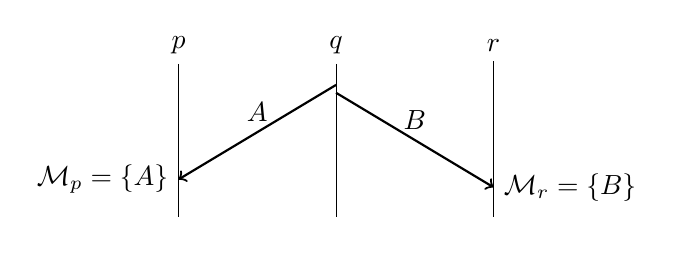
\begin{tikzpicture}
% Timelimes
\node (p-start) at (0, 0.5) {$p$};
\node (p-end)   at (0, -1.8) {};
\node (q-start) at (2, 0.5) {$q$};
\node (q-end)   at (2, -1.8) {};
\node (r-start) at (4, 0.5) {$r$};
\node (r-end)   at (4, -1.8) {};
\draw (p-start) -- (p-end);
\draw (q-start) -- (q-end);
\draw (r-start) -- (r-end);

% Messages
\draw[thick,->] (2, 0) to node [above] {$A$} (0, -1.2) node [left] {$\mathcal{M}_p = \{A\}$};

\draw[thick,->] (2, -0.1) to node [above] {$B$} (4, -1.3) node [right] {$\mathcal{M}_r = \{B\}$};

\end{tikzpicture}

    \caption{Byzantine-faulty process $q$ sends conflicting updates to correct processes $p$ and $r$.}
    \label{fig:trivial1}
\end{figure}

\begin{figure}
    \centering
    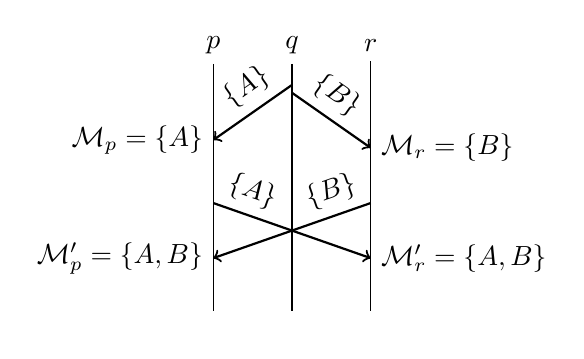
\begin{tikzpicture}

% Space between timelines
\def\width{1}
% Message delay
\def\delay{0.7}

% Timelimes
\node (p-start) at (0, 0.5) {$p$};
\node (p-end)   at (0, -3) {};
\node (q-start) at (\width, 0.5) {$q$};
\node (q-end)   at (\width, -3) {};
\node (r-start) at (\width*2, 0.5) {$r$};
\node (r-end)   at (\width*2, -3) {};
\draw (p-start) -- (p-end);
\draw (q-start) -- (q-end);
\draw (r-start) -- (r-end);

% Messages
\draw[thick,->] (\width, 0) to node [above,pos=0.4,sloped] {$\{A\}$} (0, -\delay) node [left] {$\mathcal{M}_p = \{A\}$};

\draw[thick,->] (\width, -0.1) to node [above,pos=0.4,sloped] {$\{B\}$} (\width*2, -\delay-0.1) node [right] {$\mathcal{M}_r = \{B\}$};

\draw[thick,->] (0, -1.5) to node [above,pos=0.2,sloped] {$\{A\}$} (\width*2, -1.5-\delay) node [right] {$\mathcal{M}_r' = \{A,B\}$};

\draw[thick,->] (\width*2, -1.5) to node [above,pos=0.2,sloped] {$\{B\}$} (0, -1.5-\delay) node [left] {$\mathcal{M}_p' = \{A,B\}$};

\end{tikzpicture}

% \begin{tikzpicture}
% % Timelimes
% \node (p-start) at (0, 0.5) {$p$};
% \node (p-end)   at (0, -3.4) {};
% \node (q-start) at (2, 0.5) {$q$};
% \node (q-end)   at (2, -3.4) {};
% \node (r-start) at (4, 0.5) {$r$};
% \node (r-end)   at (4, -3.4) {};
% \draw (p-start) -- (p-end);
% \draw (q-start) -- (q-end);
% \draw (r-start) -- (r-end);

% % Messages
% \draw[thick,->] (2, 0) to node [above] {$\{A\}$} (0, -1.2) node [left] {$\mathcal{M}_p = \{A\}$};

% \draw[thick,->] (2, -0.1) to node [above] {$\{B\}$} (4, -1.3) node [right] {$\mathcal{M}_r = \{B\}$};

% \draw[thick,->] (0, -1.7) to node [above,pos=0.25] {$\{A\}$} (4, -2.9) node [right] {$\mathcal{M}_r' = \{A,B\}$};

% \draw[thick,->] (4, -1.7) to node [above,pos=0.25] {$\{B\}$} (0, -2.9) node [left] {$\mathcal{M}_p' = \{A,B\}$};

% \end{tikzpicture}

    \caption{As correct processes $p$ and $r$ reconcile their sets of updates, they converge to the same set $\mathcal{U}_p' = \mathcal{U}_r' = \{A,B\}$.}
    \label{fig:trivial2}
\end{figure}

\subsection{Trivial algorithms}

The simplest replication algorithm is as follows: every time a process makes an update, it adds the update to its set $\mathcal{U}$ and broadcasts that update to every other process, re-transmitting until it is acknowledged.
Every process that receives an update also adds it to $\mathcal{U}$.
This algorithm does not converge in the face of Byzantine-faulty processes, as shown in Figure~\ref{fig:trivial1}: a faulty process $q$ may send two different updates $A$ and $B$ to correct processes $p$ and $r$, respectively.
$p$ and $r$ do not detect that they have received different updates, and so their sets of updates remain permanently inconsistent.

To detect this faulty behaviour by $q$, processes $p$ and $r$ must communicate with each other directly.
For example, as shown in Figure~\ref{fig:trivial2}, $p$ can send its entire set $\mathcal{U}_p$ to $r$, and $r$ can send $\mathcal{U}_r$ to $p$, so that both processes can compute $\mathcal{U}_p \cup \mathcal{U}_r$.
This communication can take place as a periodic \emph{reconciliation} process between every pair of processes.

Adding this reconciliation process to the replication protocol ensures BEC: all members of $\mathcal{U}$ are updates proposed by one of the processes (validity); when $p$ and $r$ reconcile their updates, they converge to the same state $\mathcal{U}_p \cup \mathcal{U}_r$ (convergence); and periodic reconciliation ensures that any two processes eventually exchange their updates (liveness).

However, this algorithm is very inefficient.
When processes periodically reconcile their state, we can expect that at the start of each round of reconciliation their sets of updates already have many elements in common.
Sending the entire set of updates to each other thus implies transmitting a large amount of data unnecessarily.

A more efficient reconciliation algorithm should determine which elements the processes' sets already have in common, and transmit only those updates that are unknown to the other process.
For example, $p$ should only send $\mathcal{U}_p - \mathcal{U}_r$ to $r$, and $r$ should only send $\mathcal{U}_r - \mathcal{U}_p$ to $p$.

\begin{figure}
    \centering
    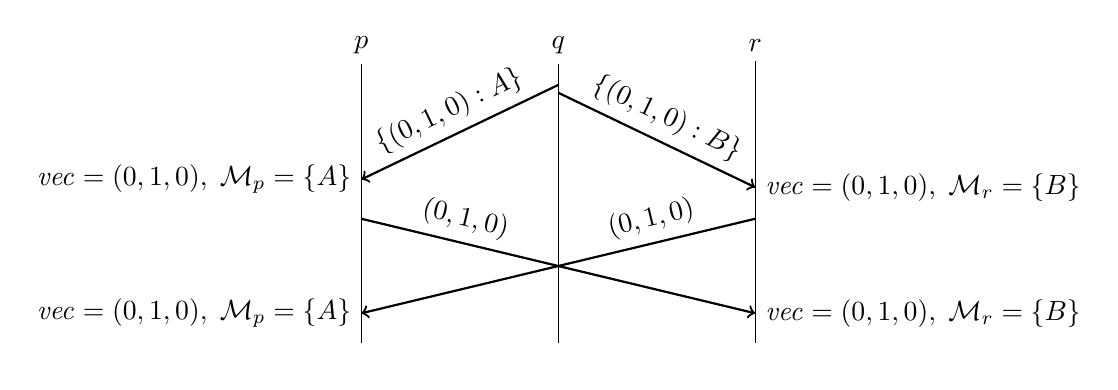
\begin{tikzpicture}
% Timelimes
\node (p-start) at (0, 0.5) {$p$};
\node (p-end)   at (0, -3.4) {};
\node (q-start) at (2.5, 0.5) {$q$};
\node (q-end)   at (2.5, -3.4) {};
\node (r-start) at (5, 0.5) {$r$};
\node (r-end)   at (5, -3.4) {};
\draw (p-start) -- (p-end);
\draw (q-start) -- (q-end);
\draw (r-start) -- (r-end);

% Messages
\draw[thick,->] (2.5, 0) to node [above,sloped] {$\{(0,1,0): A\}$} (0, -1.2) node [left] {$\mathit{vec} = (0,1,0),\; \mathcal{M}_p = \{A\}$};

\draw[thick,->] (2.5, -0.1) to node [above,sloped] {$\{(0,1,0): B\}$} (5, -1.3) node [right] {$\mathit{vec} = (0,1,0),\; \mathcal{M}_r = \{B\}$};

\draw[thick,->] (0, -1.7) to node [above,pos=0.25,sloped] {$(0,1,0)$} (5, -2.9) node [right] {$\mathit{vec} = (0,1,0),\; \mathcal{M}_r = \{B\}$};

\draw[thick,->] (5, -1.7) to node [above,pos=0.25,sloped] {$(0,1,0)$} (0, -2.9) node [left] {$\mathit{vec} = (0,1,0),\; \mathcal{M}_p = \{A\}$};

\end{tikzpicture}

    \caption{Processes $p$ and $r$ believe to be in the same state because their vector timestamps are the same, when in fact their sets of updates are inconsistent due to $q$'s faulty behaviour.}
    \label{fig:vectorclocks}
\end{figure}

\subsection{Vector clocks}

Non-Byzantine replication algorithms often rely on \emph{vector clocks} or \emph{version vectors} to determine which updates to send to each other~\cite{Ahamad:1995,Lloyd:2011,Schwarz:1994}.
However, vector clocks are not suitable in a Byzantine setting.
The problem is illustrated in Figure~\ref{fig:vectorclocks}, where faulty process $q$ generates two different updates, $A$ and $B$, with the same vector timestamp $(0, 1, 0)$.

In a system where processes correctly follow the protocol, the three components of the timestamp represent the number of updates generated by $p$, $q$, and $r$ respectively.
Thus, $p$ and $r$ should be able to reconcile their updates by first sending each other their latest vector timestamps, which serve as a concise summary of the set of updates they have seen.
However, in the example of Figure~\ref{fig:vectorclocks}, this approach fails due to $q$'s earlier faulty behaviour: $p$ and $r$ detect that their vector timestamps are equal, and thus incorrectly believe that they are in the same state, even though their sets of updates are different.

Since a vector clock can thus be corrupted by a faulty process, a BEC reconciliation algorithm must find a different way of summarising sets of updates that is not vulnerable to such corruption.

\subsection{An efficient BEC reconciliation algorithm}

We now present a reconciliation algorithm that can be run by any two replicas to bring their sets of updates into the same state.
Our algorithm is efficient in the sense that when two correct processes are communicating, one process does not send any updates that the other process already has.
We prove in \S~\ref{sec:proof} that this algorithm ensures BEC, regardless of the number of Byzantine-faulty processes in the system.

Let the set of updates $\mathcal{U}$ be a set of pairs $(v, \mathit{hs})$, where $v$ is any value, and $\mathit{hs}$ is a set of hashes produced by a cryptographic hash function $H(\cdot)$, such as SHA-256.
We assume that $H$ is collision-resistant, i.e.\ that it is computationally infeasible to find distinct $x$ and $y$ such that $H(x) = H(y)$.

Say $\mathcal{U}$ contains updates $A = (v_A, \mathit{hs}_A)$ and $B = (v_B, \mathit{hs}_B)$, where $H(A) \in \mathit{hs}_B$.
Then we call $A$ a \emph{predecessor} of $B$, and $B$ a \emph{successor} of $A$.
Define a graph with a vertex for each update in $\mathcal{U}$, and a directed edge from each update to each of its predecessors.
We can assume that this graph is acyclic because the presence of a cycle would imply knowledge of a collision in the hash function.
Fig.~\ref{fig:example-dags} shows examples of such graphs.

Let $\mathrm{succ}^1(\mathcal{U}, u)$ be the set of successors of update $u$ in $\mathcal{U}$, let $\mathrm{succ}^2(\mathcal{U}, u)$ be the successors of the successors of $u$, and so on, and define $\mathrm{succ}^*(\mathcal{U}, u)$ to be the transitive closure:
\[
\mathrm{succ}^i(\mathcal{U}, u) =
\begin{cases}
\{( v, \mathit{hs}) \in \mathcal{U} \mid H(u) \in \mathit{hs}\} & \text{ for } i=1 \\
\bigcup_{u' \in \mathrm{succ}^1(\mathcal{U}, u)} \mathrm{succ}^{i-1}(\mathcal{U}, u') & \text{ for } i>1
\end{cases}
\hspace{30pt}
\mathrm{succ}^*(\mathcal{U}, u) = \bigcup_{i \ge 1} \mathrm{succ}^i(\mathcal{U}, u)
\]

Let $\mathrm{heads}(\mathcal{U})$ denote the set of hashes of updates in $\mathcal{U}$ that have no successors:
\[ \mathrm{heads}(\mathcal{U}) = \{H(u) \mid u \in \mathcal{U} \wedge \mathrm{succ}^1(\mathcal{U}, u) = \{\}\;\}. \]

We define the reconciliation process as taking place over a \emph{connection}.
This connection is a logical grouping of a bidirectional sequence of related messages between two processes (in practice, it can be implemented as a TCP connection).
Connections have the same reliability assumptions as individual message delivery: messages may be dropped, resulting in the connection eventually timing out, and the reconciliation process being cancelled.
For liveness purposes we assume that if two processes repeatedly try, eventually they will succeed in creating a connection of finite duration that is free from message loss.

When one process connects to another, both processes execute Algorithm~\ref{fig:algorithm}.
We will illustrate the operation of this algorithm using the example in Fig.~\ref{fig:example-dags}; the messages sent in the course of the execution are shown in Fig.~\ref{fig:messages}.

\begin{figure}[p]
    \centering
    \begin{subfigure}{0.45\textwidth}
    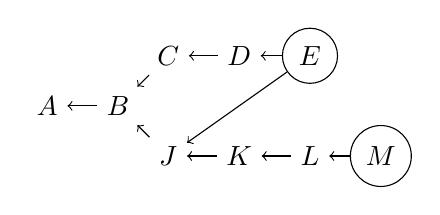
\begin{tikzpicture}[node distance=0.9cm]

% nodes
\node (a) {$A$};
\node (b) [right of=a] {$B$};
\node (c) [above right of=b] {$C$};
\node (d) [right of=c] {$D$};
\node (e) [right of=d,draw,circle] {$E$};
\node (j) [below right of=b] {$J$};
\node (k) [right of=j] {$K$};
\node (l) [right of=k] {$L$};
\node (m) [right of=l,draw,circle] {$M$};

% arrows
\draw[<-] (a) -- (b);
\draw[<-] (b) -- (c);
\draw[<-] (c) -- (d);
\draw[<-] (d) -- (e);
\draw[<-] (j) -- (e);
\draw[<-] (b) -- (j);
\draw[<-] (j) -- (k);
\draw[<-] (k) -- (l);
\draw[<-] (l) -- (m);
\end{tikzpicture}
    \caption{Graph of updates at $p$ before reconciliation}
    \end{subfigure}\hfill
    \begin{subfigure}{0.45\textwidth}
    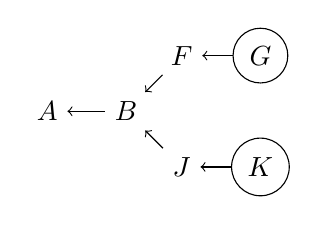
\begin{tikzpicture}

% nodes
\node (a) {$A$};
\node (b) [right of=a] {$B$};
\node (f) [above right of=b] {$F$};
\node (g) [right of=f,circle,draw] {$G$};
\node (j) [below right of=b] {$J$};
\node (k) [right of=j,circle,draw] {$K$};

% arrows
\draw[<-] (a) -- (b);
\draw[<-] (b) -- (f);
\draw[<-] (f) -- (g);
\draw[<-] (b) -- (j);
\draw[<-] (j) -- (k);
\end{tikzpicture}
    \caption{Graph of updates at $q$ before reconciliation}
    \end{subfigure}\\[10pt]
    \begin{subfigure}{0.4\textwidth}
    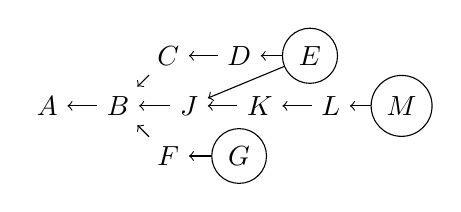
\begin{tikzpicture}[node distance=0.9cm]

% nodes
\node (a) {$A$};
\node (b) [right of=a] {$B$};
\node (c) [above right of=b] {$C$};
\node (d) [right of=c] {$D$};
\node (e) [right of=d,draw,circle] {$E$};
\node (j) [right of=b] {$J$};
\node (k) [right of=j] {$K$};
\node (l) [right of=k] {$L$};
\node (m) [right of=l,draw,circle] {$M$};
\node (f) [below right of=b] {$F$};
\node (g) [right of=f,draw,circle] {$G$};

% arrows
\draw[<-] (a) -- (b);
\draw[<-] (b) -- (c);
\draw[<-] (c) -- (d);
\draw[<-] (d) -- (e);
\draw[<-] (b) -- (j);
\draw[<-] (j) -- (e);
\draw[<-] (j) -- (k);
\draw[<-] (k) -- (l);
\draw[<-] (l) -- (m);
\draw[<-] (b) -- (f);
\draw[<-] (f) -- (g);
\end{tikzpicture}
    \caption{Graph of updates at $p$ and $q$ after reconciliation}
    \end{subfigure}
    \caption{Example DAGs of updates. Arrows represent an update referencing the hash of its predecessor, and heads (updates with no successors) are marked with circles.}
    \label{fig:example-dags}
\end{figure}

\begin{figure}[p]
    \vspace{0.5cm}
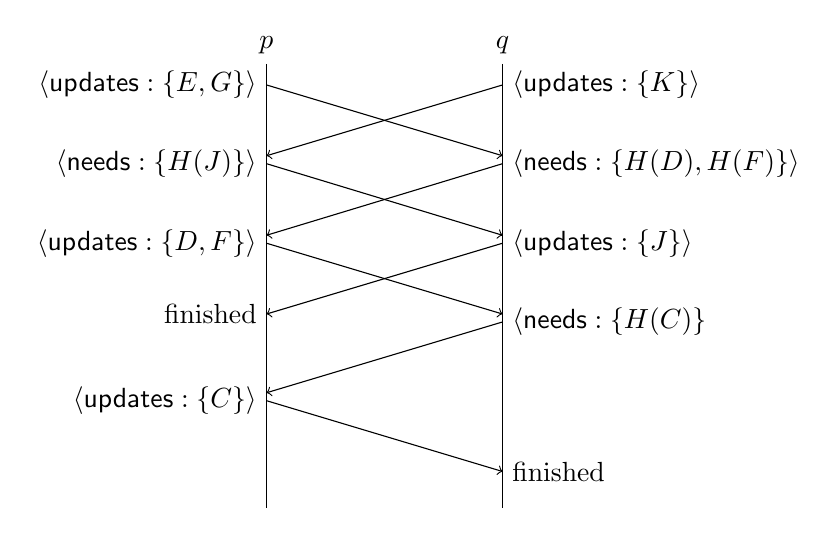
\begin{tikzpicture}
\def\width{3cm}
\def\latency{1cm}
\def\spacing{0.1cm}
\def\length{6cm}
\def\startdelay{0.5cm}

% Timelimes
\node (p1-start) at (0,0) {$p$};
\node (p2-start) at (\width,0) {$q$};
\node (p1-end) at (0,-\length) {};
\node (p2-end) at (\width,-\length) {};
\draw (p1-start) -- (p1-end);
\draw (p2-start) -- (p2-end);

% Messages
\draw[->] (0,-\startdelay) node[left] {$\langle\mathsf{updates}: \{E,G\}\rangle$} -- (\width,\spacing-\startdelay-\latency);
\draw[->] (\width,-\startdelay) node[right] {$\langle\mathsf{updates}: \{K\}\rangle$} -- (0,\spacing-\startdelay-\latency);

\draw[->] (\width, -\startdelay-\latency) node[right] {$\langle\mathsf{needs}: \{H(D), H(F)\}\rangle$} -- (0,\spacing-\startdelay-2.0\latency);
\draw[->] (0, -\startdelay-\latency) node[left] {$\langle\mathsf{needs}: \{H(J)\}\rangle$} -- (\width,\spacing-\startdelay-2.0\latency);

\draw[->] (0, -\startdelay-2.0\latency) node[left] {$\langle\mathsf{updates}: \{D, F\}\rangle$} -- (\width,\spacing-\startdelay-3.0\latency);
\draw[->] (\width, -\startdelay-2.0\latency) node[right] {$\langle\mathsf{updates}: \{J\}\rangle$} -- (0,\spacing-\startdelay-3.0\latency) node[left] {finished};

\draw[->] (\width, -\startdelay-3.0\latency) node[right] {$\langle\mathsf{needs}: \{H(C)\}$} -- (0,\spacing-\startdelay-4.0\latency);

\draw[->] (0, -\startdelay-4.0\latency) node[left] {$\langle\mathsf{updates}: \{C\}\rangle$} -- (\width,\spacing-\startdelay-5.0\latency) node[right] {finished};

\end{tikzpicture}
    \caption{Messages sent in the course of running the reconciliation process in Algorithm~\ref{fig:algorithm} with the example in Figure~\ref{fig:example-dags}.}
    \label{fig:messages}
\end{figure}

\begin{algorithm}[p]
    \algblockdefx{On}{EndOn}[1]{\textbf{on} #1 \textbf{do}}{\textbf{end on}}
    \begin{algorithmic}[1]
    \On{connecting to another process}
        \State $\mathit{sent} := \{\};\; \mathit{received} := \{\};\; \mathcal{U}_\mathsf{conn} := \mathcal{U}$ \label{line:init}\Comment{connection-local variables}
        \State \textbf{send} $\langle\mathsf{heads}: \mathrm{heads}(\mathcal{U}_\mathsf{conn})\rangle$ \label{line:send-heads}
    \EndOn
    \State
    \On{receiving $\langle\mathsf{heads}: \mathit{hs}\rangle$} \label{line:recv-heads}
        \State $\mathit{reply} := \{v \mid \exists u \in \mathcal{U}_\mathsf{conn}.\; H(u) \in \mathit{hs} \,\wedge\, v \in \mathrm{succ}^*(\mathcal{U}_\mathsf{conn}, u)\}$ \label{line:succ}
        \If{$\mathit{reply} \neq \{\}$}
            \State $\mathit{sent} := \mathit{sent} \cup \mathit{reply}$
            \State \textbf{send} $\langle\mathsf{updates}: \mathit{reply}\rangle$ \label{line:heads-reply}
        \EndIf
        \State \Call{HandleMissing}{$\{h \in \mathit{hs} \mid \nexists u \in \mathcal{U}_\mathsf{conn}.\; H(u) = h\}$} \label{line:heads-missing}
    \EndOn
    \State
    \On{receiving $\langle\mathsf{updates}: \mathit{new}\rangle$} \label{line:recv-updates}
        \State $\mathit{received} := \mathit{received} \,\cup\, \mathit{new}$ \label{line:updates-received}
        \State $\mathit{missing} := \{h \mid \exists (v, \mathit{hs}) \in \mathit{received}.\; h \in \mathit{hs} \;\wedge\; \nexists u \in (\mathcal{U}_\mathsf{conn} \cup \mathit{received}).\; H(u) = h\}$ \label{line:updates-missing}
        \State \Call{HandleMissing}{$\mathit{missing}$} \label{line:updates-handle-missing}
    \EndOn
    \State
    \On{receiving $\langle\mathsf{needs}: \mathit{missing}\rangle$} \label{line:recv-needs}
        \State $\mathit{reply} := \{u \in \mathcal{U}_\mathsf{conn} \mid H(u) \in \mathit{missing} \wedge u \notin \mathit{sent}\}$ \label{line:needs-reply}
        \State $\mathit{sent} := \mathit{sent} \cup \mathit{reply}$
        \State \textbf{send} $\langle\mathsf{updates}: \mathit{reply}\rangle$ \label{line:send-updates}
    \EndOn\label{line:end-needs}
    \State
    \Function{HandleMissing}{$\mathit{missing}$}
        \If{$\mathit{missing} = \{\}$} \label{line:missing-empty}
            \State $\mathcal{U} := \mathcal{U} \cup \mathit{received}$ \label{line:update-u}
            \State \textbf{reconciliation complete} \label{line:finish}
        \Else
            \State \textbf{send} $\langle\mathsf{needs}: \mathit{missing}\rangle$ \label{line:send-missing}
        \EndIf
    \EndFunction
    \end{algorithmic}
    \caption{A reconciliation algorithm to sync updates between two processes.}\label{fig:algorithm}
\end{algorithm}

Initially, when a connection is established between two processes, they send each other their heads (Algorithm~\ref{fig:algorithm}, line~\ref{line:send-heads}).
In the example of Fig.~\ref{fig:example-dags}, $p$ sends $\{H(E),H(M)\}$ to $q$, while $q$ sends $\{H(G),H(K)\}$ to $p$.

Each process also initialises variables $\mathit{sent}$ and $\mathit{received}$ to contain the set of updates sent to/received from the other process within the scope of this particular connection, and $\mathcal{U}_\mathsf{conn}$ contains a copy of this process' set of updates $\mathcal{U}$ at the time the connection is established (line~\ref{line:init}).
A process may concurrently execute several instances of this algorithm using several connections; in this case, each connection has a separate copy of the variables $\mathit{sent}$, $\mathit{received}$, and $\mathcal{U}_\mathsf{conn}$.

On receiving the heads from the other process (line~\ref{line:recv-heads}), the recipient first checks if its local set $\mathcal{U}_\mathsf{conn}$ contains successors for any of the sender's heads; if so, those successors, and any transitive successors, are sent immediately to the other process (lines~\ref{line:succ}--\ref{line:heads-reply}).
By definition of $\mathit{heads}$, these successors are not yet known to the other process.

If the recipient does not know some of the head hashes, it replies with a $\mathsf{needs}$ message requesting the updates matching those hashes (lines~\ref{line:heads-missing}, \ref{line:send-missing}).
A process responds to such a $\mathsf{needs}$ message by returning all the matching updates (lines~\ref{line:recv-needs}--\ref{line:end-needs}).
That $\mathsf{updates}$ message might again contain unresolved hashes, resulting in another $\mathsf{needs}$ message (lines~\ref{line:updates-missing}--\ref{line:updates-handle-missing}).
In successive rounds of this protocol, the processes work their way from the heads along the paths of predecessors, until they reach the updates that are common ancestors of both processes' heads.

Eventually, when there are no unresolved hashes, we merge the set of received updates into $\mathcal{U}$ and conclude the protocol run (lines~\ref{line:missing-empty}--\ref{line:finish}).
This is the moment at which the ``reconciliation is complete'', as per the convergence property of Byzantine Eventual Consistency.
We show in \S~\ref{sec:proof} that this algorithm satisfies all three properties of BEC.

\subsection{Optimisations and extensions}\label{sec:optimisations}

Assuming that the number of heads is small compared to the total number of updates in $\mathcal{U}$, the initial $\mathsf{heads}$ message will be small, yielding a big performance improvement over sending the whole of $\mathcal{U}$.

In order to keep the number of heads small, whenever a correct process generates a new update $(v, \mathit{hs})$, it should set $\mathit{hs}$ to be the set of hashes of the current heads:
$\mathit{hs} = \mathrm{heads}(\mathcal{U})$.
In this construction, the number of heads is bounded by the number of processes generating updates concurrently.
A Byzantine-faulty process may generate a large number of heads, which will affect the performance of the algorithm, but not its correctness.

A downside of Algorithm~\ref{fig:algorithm} is that the number of round trips required can be up to the length of the longest path in the graph.
In order to optimise this, we could change lines~\ref{line:needs-reply}--\ref{line:send-updates} to send not only the immediate updates identified by the hashes in the $\mathsf{needs}$ message, but also all of the predecessors of those updates, several levels deep.
The number of round-trips is then reduced proportionally to the number of predecessor levels, but the downside is that some of the predecessor updates may already be known to the recipient, and are thus transmitted unnecessarily.

To determine the number of predecessor levels to send in each round, as a rule of thumb, the size of the $\mathsf{updates}$ message should be approximately equal to the bandwidth-delay product of the connection between the two processes.
Thus, on a connection with low bandwidth and fast round-trips we will prefer to send many small messages, while on a connection with high bandwidth and slow round-trips we will batch the updates into a small number of large messages.

In order to further improve efficiency, the processes can send each other a probabilistic data structure summarising the set of elements in their local set $\mathcal{U}$, such as a Bloom filter~\cite{Bloom:1970}.
The recipient of such a structure can then compute the approximate set of updates that the other process is missing; however, this set may be incomplete due to false positives, necessitating at least one more round trip of communication to fill in the gaps.
A detailed study of the performance characteristics of this approach is beyond the scope of this paper.

Another potential issue with Algorithm~\ref{fig:algorithm} is the unbounded growth of storage requirements, since the set $\mathcal{U}$ grows monotonically (much like most algorithms for Byzantine agreement, which produce an append-only log without considering how that log might be truncated).
If the set of processes in the system is known, we can perform garbage collection in the set $\mathcal{U}$ using the following observation: once some update $u$ is known to all of the processes, Algorithm~\ref{fig:algorithm} no longer needs to refer to any of the predecessors of $u$, and so all of those predecessors can be removed from $\mathcal{U}$ without affecting the algorithm.

Some systems may need to check the authenticity of updates (i.e.\ to verify that an update was generated by a particular process).
This can easily be achieved by attaching a digital signature to each update.

% reuse prior knowledge of other processes

% Find last common ancestor by some kind of binary search; problem: graph of updates is not linear, so definition of half-way point is fiddly.

\subsection{Building applications on top of BEC}\label{sec:applications}

BEC can ensure convergence for any data structure that is a deterministic function of the set of updates $\mathcal{U}$.
For example, we can implement Byzantine eventually consistent state machine replication (BEC-SMR) as follows: let each value in $\mathcal{U}$ be a pair $(t, \mathit{op})$, where $t$ is a timestamp and $\mathit{op}$ is a state machine operation.
Any process may propose an operation $op$ to add to the log by generating $t$ and adding $((t, \mathit{op}), \mathit{hs})$ to $\mathcal{U}$.
The log is then simply the sequence of operations obtained by sorting the elements of $\mathcal{U}$ by timestamp, breaking ties by ordering on the hash of the respective update.

Unlike the log produced by Byzantine agreement, the BEC-SMR log does not guarantee that operations are added to the log in increasing timestamp order.
Thus, if a process receives operations out-of-order, it may need to roll back the state machine to an earlier state, and then replay operations in timestamp order.

This rollback approach is only feasible if all side-effects of the state machine can be undone~\cite{Jefferson:1985}.
If side-effects need to be irrevocable, BEC-SMR is not suitable, and a traditional Byzantine agreement algorithm must be used.
For example, most blockchains require that a payment (a side-effect of processing a block) cannot be reversed once it has been confirmed by the consensus algorithm.

\section{Proof of correctness}\label{sec:proof}

In this section we show that the reconciliation algorithm of \S~\ref{sec:algorithm} satisfies the properties of Byzantine Eventual Consistency.

We consider two correct processes $p$ and $q$, with initial sets of updates $\mathcal{U}_p$ and $\mathcal{U}_q$ respectively at the start of the execution.
Assume that in this run of the algorithm, $p$ and $q$ both complete the reconciliation by reaching line~\ref{line:finish} of Algorithm~\ref{fig:algorithm}.
Let $\mathit{received}_p$ be the contents of the variable $\mathit{received}$ at process $p$ when the reconciliation is complete, and likewise $\mathit{received}_q$ at process $q$.
Further, let $\mathcal{U}'_p = \mathcal{U}_p \cup \mathit{received}_p$ and $\mathcal{U}'_q = \mathcal{U}_q \cup \mathit{received}_q$ be the final set of updates at both processes.

\begin{lemma}\label{lemma:no-p-missing}
The set of updates $\mathcal{U}$ of a correct process $p$ grows monotonically.
\end{lemma}
\begin{proof}
The process $p$ only modifies $\mathcal{U}$ by unioning it with the set $\mathit{received}$ (Algorithm~\ref{fig:algorithm}, line~\ref{line:update-u}), or by generating new operations, which are added to $\mathcal{U}$.
Thus, elements are only added to the set $\mathcal{U}$, and therefore $\mathcal{U}$ grows monotonically.
\end{proof}

\begin{lemma}\label{lemma:no-dangling}
Let $u = (\mathit{val}, \mathit{hs})$ such that $u \in \mathcal{U}_p$.
Then $\forall h \in \mathit{hs}.\; \exists v \in \mathcal{U}_p.\; H(v) = h$.
\end{lemma}
\begin{proof}
There are two ways how $u$ can become a member of $\mathcal{U}_p$ for a correct process $p$:
\begin{enumerate}
    \item $u$ is generated by process $p$.
    In this case, since $p$ is assumed to be correct, $\mathit{hs} = \{H(v) \mid v \in \mathcal{U} \wedge \mathrm{succ}^1(\mathcal{U}, v) = \{\}\,\}$ for some earlier state $\mathcal{U}$, as per \S~\ref{sec:optimisations}.
    As $\mathcal{U}$ grows monotonically (Lemma~\ref{lemma:no-p-missing}), $\mathcal{U} \subseteq \mathcal{U}_p$, and thus we can deduce that $\forall h \in \mathit{hs}.\; \exists v \in \mathcal{U}_p.\; H(v) = h$.
    \item $u$ is received during reconciliation with another process (which might be faulty).
    In this case, during the run of the protocol at which $p$ received $u$, we have $u \in \mathit{received}$ and $\mathit{missing} = \{\}$ at line~\ref{line:update-u} of Algorithm~\ref{fig:algorithm}.
    Let $\mathcal{U}$ be the set of updates at $p$ immediately before that execution of line~\ref{line:update-u}.
    From $\mathit{missing} = \{\}$ and line~\ref{line:updates-missing} we can deduce that $\forall h \in \mathit{hs}.\; \exists v \in (\mathcal{U} \cup \mathit{received}).\; H(v) = h$.
    Since $\mathcal{U}$ grows monotonically (Lemma~\ref{lemma:no-p-missing}) and $\mathit{received} \subseteq \mathcal{U}_p$ (line~\ref{line:update-u}) we have $\forall h \in \mathit{hs}.\; \exists v \in \mathcal{U}_p.\; H(v) = h$.
\end{enumerate}
\end{proof}

\begin{lemma}\label{lemma:no-collision}
Let $u = (\mathit{val}, \mathit{hs})$ such that $u \in \mathcal{U}_p$ and $u \in \mathcal{U}_q$.
Then $\{v \in \mathcal{U}_p \mid H(v) \in \mathit{hs}\} = \{v \in \mathcal{U}_q \mid H(v) \in \mathit{hs}\}$.
\end{lemma}
\begin{proof}
We use proof by contradiction.\\
Assume there exists $h \in \mathit{hs}$ such that $\{v \in \mathcal{U}_p \mid H(v) = h\} \neq \{v \in \mathcal{U}_q \mid H(v) = h\}$.\\
From Lemma~\ref{lemma:no-dangling} we have that $\{v \in \mathcal{U}_p \mid H(v) = h\} \neq \{\}$ and $\{v \in \mathcal{U}_q \mid H(v) = h\} \neq \{\}$.\\
Hence, there exist $v \in \mathcal{U}_p$ and $v' \in \mathcal{U}_q$ such that $v \neq v'$ and $H(v) = H(v') = h$.\\
However, this contradicts our assumption in \S~\ref{sec:algorithm} that the hash function $H(\cdot)$ is collision-resistant.
\end{proof}

\begin{lemma}\label{lemma:no-q-missing}
$\mathcal{U}_q \subseteq \mathcal{U}'_p$
\end{lemma}
\begin{proof}
We use proof by contradiction.\\
Assume that $\exists u \in \mathcal{U}_q.\; u \notin  \mathcal{U}'_p$.\\
Since $\mathit{received} \subseteq \mathcal{U}'_p$ and elements are only added to $\mathit{received}$ (Algorithm~\ref{fig:algorithm}, line~\ref{line:updates-received}) then $u \notin  \mathcal{U}'_p$ implies that $u \notin \mathit{received}$ on process $p$.\\
Since $u \in \mathcal{U}_q$ we have either $\mathrm{succ}^1(\mathcal{U}_q, u) = \{\}$ or $\mathrm{succ}^1(\mathcal{U}_q, u) \ne \{\}$, and we now consider each case in turn.
\begin{enumerate}
    \item\textsc{Case} $\mathrm{succ}^1(\mathcal{U}_q, u) = \{\}$:\\
    In this case, $H(u) \in \mathrm{heads}(\mathcal{U}_q)$, and so the first $\mathsf{heads}$ message from $q$ to $p$ will contain $H(u)$ (Algorithm~\ref{fig:algorithm}, line~\ref{line:send-heads}).\\
    Since $u \notin \mathcal{U}_p$, process $p$ will send a $\mathsf{needs}$ message to $q$ containing $H(u)$ (Algorithm~\ref{fig:algorithm}, line~\ref{line:heads-missing}).\\
    Upon receiving the $\mathsf{needs}$ message containing $H(u)$, process $q$ will reply with an $\mathsf{updates}$ message containing $u$ (Algorithm~\ref{fig:algorithm}, line~\ref{line:send-updates}).\\
    Process $p$ will receive the $\mathsf{updates}$ message with $u$ from process $q$ and will add $u$ to $\mathit{received}$ (Algorithm~\ref{fig:algorithm}, line~\ref{line:updates-received}).\\
    This contradicts our previous finding that $u \notin \mathit{received}$.
    
    \item\textsc{Case} $\mathrm{succ}^1(\mathcal{U}_q, u) \ne \{\}$:\\
    In this case, $H(u) \notin \mathrm{heads}(\mathcal{U}_q)$.
    Since $\mathcal{U}_q$ is a DAG, there must exist an update $v$ such that $H(v) \in \mathrm{heads}(\mathcal{U}_q)$ and $v \in \mathrm{succ}^*(\mathcal{U}_q, u)$.\\
    As in the previous case, $H(v) \in \mathrm{heads}(\mathcal{U}_q)$ implies that $v \in \mathit{received}$.\\
    Note that none of the updates in $\mathrm{succ}^*(\mathcal{U}_q, u)$ are in $\mathcal{U}_p$ as $u \notin \mathcal{U}'_p$ implies that  $u \notin \mathcal{U}_p$ (Lemma~\ref{lemma:no-p-missing}).\\
    If $v \in \mathrm{succ}^1(\mathcal{U}_q, u)$ then it must the case that $u \in \mathit{received}$ by the time that $\mathit{missing} = \emptyset$, otherwise $u \in \mathit{missing}$ (Algorithm~\ref{fig:algorithm}, line~\ref{line:updates-missing}).\\
    By induction over the path of successors from $v$ to $u$, we observe that $u \in \mathit{received}$.\\
    At each step of the induction, the processes move to the predecessors of the previous step; due to Lemma~\ref{lemma:no-collision}, $p$ and $q$ agree about the identity of these predecessors.\\
    This contradicts our previous finding that $u \notin \mathit{received}$.
\end{enumerate}
\end{proof}

\begin{lemma}\label{lemma:no-extras}
$\mathcal{U}'_p \subseteq \mathcal{U}_p \cup \mathcal{U}_q$    
\end{lemma}
\begin{proof}
We use proof by contradiction.\\
Assume that $\exists u \in \mathcal{U}'_p.\; u \notin \mathcal{U}_p  \land  u \notin \mathcal{U}_q$.\\
Since $\exists u \in \mathcal{U}'_p$, the process $p$ must have received an update containing $u$ from process $q$ before it completed reconciliation (Algorithm~\ref{fig:algorithm}, lines \ref{line:recv-updates}, \ref{line:updates-received}, \ref{line:finish}).\\
Process $q$ will only send an update containing $u$ if $u \in \mathcal{U}_q$ or $u \in \mathcal{U}'_q$, depending on whether process $q$ has completed the reconciliation algorithm.
Since $u \notin \mathcal{U}_q$ then process $q$ must have received an update containing $u$ from process $p$.
Since $u \notin \mathcal{U}_p$ then process $p$ will not send this message and therefore the update $u$ does not exist.
\end{proof}

\begin{theorem}\label{theorem:convergence}
When two correct processes $p$ and $q$, with initial sets of updates $\mathcal{U}_p$ and $\mathcal{U}_q$, have completed reconciliation (i.e.\ both have reached line~\ref{line:finish} of Algorithm~\ref{fig:algorithm}), then their final sets of updates $\mathcal{U}'_p$ and $\mathcal{U}'_q$  are both equal to $\mathcal{U}_q \cup \mathcal{U}_q$.
\end{theorem}
\begin{proof}
We can prove that $\mathcal{U}'_p = \mathcal{U}_q \cup \mathcal{U}_q$ by showing the following:
\begin{enumerate}
   \item $\mathcal{U}_p \subseteq \mathcal{U}'_p$
   \item $\mathcal{U}_q \subseteq \mathcal{U}'_p$
   \item $\mathcal{U}'_p \subseteq \mathcal{U}_p \cup \mathcal{U}_q$
\end{enumerate}

These have been shown by lemmas \ref{lemma:no-p-missing}, \ref{lemma:no-q-missing} and \ref{lemma:no-extras} respectively.  
By swapping $p$ and $q$, we can show that the same holds for $\mathcal{U}'_q$.
\end{proof}

This concludes the proof that the reconciliation algorithm of \S~\ref{sec:algorithm} satisfies the convergence property of BEC.
The proof of the validity property is obvious (the only way how an update in $\mathcal{U}$ can come into existence is by being proposed by one of the processes).
It remains only to show the liveness property:

\begin{theorem}\label{theorem:liveness}
Assuming that any two correct processes execute the reconciliation protocol an unbounded number of times, and assuming that only a finite number of messages are lost, an update proposed by one process will eventually be in the set of updates for all correct processes.
\end{theorem}
\begin{proof}
Since the graph of updates $\mathcal{U}_p$ at any correct process $p$ is finite and contains no cycles, every vertex $v \in \mathcal{U}_p$ can be reached in a finite number of steps by starting a graph traversal at $\mathrm{heads}(\mathcal{U}_p)$ and, in each step, moving from each vertex to its predecessors.
Since $\mathcal{U}_p$ at any correct process $p$ contains only hashes that are the hash of another update in $\mathcal{U}_p$ (Lemma~\ref{lemma:no-dangling}), the algorithm of Algorithm~\ref{fig:algorithm} will always reach the state $\mathit{missing} = \{\}$ and terminate (i.e.\ reach line~\ref{line:finish} of Algorithm~\ref{fig:algorithm}) in a finite number of round-trips of $\mathsf{needs}$ and $\mathsf{updates}$ messages, when communicating with another correct process.

Since we assume that only a finite number of messages are ever lost, there will be an infinite number of executions of the protocol for any two correct processes $p$ and $q$ in which no messages are lost.
In those protocol runs in which all messages are delivered, $p$ and $q$ will both complete in a finite time, because each of the finite number of round-trips completes in finite time.
Thus, by Theorem~\ref{theorem:convergence}, any update known to $p$ will eventually be known to $q$ and vice versa.
\end{proof}

Note that the protocol may never terminate when one of the communicating processes is Byzantine-faulty, e.g.\ because the faulty process may send hashes that do not resolve to any update, and so the state $\mathit{missing} = \{\}$ is never reached.
However, in a non-terminating protocol run $\mathcal{U}$ is never updated, and so the actions of the faulty process have no effect on the state of the correct process.

In a protocol run that terminates, the only things a Byzantine-faulty process can do is to omit heads, or to extend the set $\mathcal{U}$ with well-formed updates (i.e.\ updates containing only hashes that resolve to other updates).
If a faulty process responds incorrectly to a $\mathsf{needs}$ message, likewise any effects on the recipient's state are limited to well-formed updates.
This ensures the integrity of the DAG.
Arbitrary $\mathsf{needs}$ messages sent by a faulty process have no consequence, since they do not affect the state of the recipient.
Thus, a faulty process cannot corrupt the state of a correct process in a way that would prevent the correct process from later synchronising its set of updates with another correct process.

\section{Related Work}

Byzantine agreement has been subject of extensive research and has seen a recent renewal of interest due to its application in permissioned blockchains~\cite{Bano:2019}.
Many Byzantine agreement algorithms~\cite{Castro:1999,Kotla:2007,Bessani:2014,Aublin:2015,Cowling:2006,Abd:2005} for asynchronous environments assume $n \ge 3f+1$ and require at least one round of communication with at least $2f+1$ processes, incurring both significant latency and limiting availability.
Zeno~\cite{Singh:2009} makes progress with just $f+1$ processes, but safety depends on less than $\frac{1}{3}$ of processes being Byzantine-faulty.
Byzec~\cite{Shoker:2017}, as well as work by Chai and Zhao~\cite{Chai:2014}, also considers eventual consistency in the context of Byzantine faults but again assumes that $f$ of $3f+1$ processes are faulty.

Depot~\cite{Mahajan:2011} tolerates arbitrary numbers of faulty processes; however, its consistency model (fork-join-causal) and replication protocol are considerably more complicated than ours, making them difficult to analyse.
In BFT2F~\cite{Li:2007} and SUNDR~\cite{Mazieres:2002}, a faulty process can partition the system, preventing some processes from ever synchronising again.

Byzantine Eventual Consistency is based on \emph{Strong Eventual Consistency} (SEC)~\cite{Shapiro:2011}, a non-Byzantine consistency model in which replicas eventually converge towards the same state.
Conflict-free Replicated Data Types (CRDTs) provide SEC by ensuring that whenever any two replicas have seen the same set of updates (possibly in a different order), those replicas are in the same state~\cite{Shapiro:2011}.
We can strengthen CRDTs to provide Byzantine Eventual Consistency by making each operation an update, and using the algorithm of \S~\ref{sec:algorithm} to reconcile the sets of operations.

The hash chaining approach of our algorithm resembles a Git commit history, a blockchain~\cite{Bano:2019}, or a Merkle tree~\cite{Merkle:1987}.
Our algorithm in \S~\ref{sec:algorithm} has similarities to the protocol used by \texttt{git fetch}~\cite{GitHTTP}.
However, to our knowledge the Git protocol has not yet been the subject of much study, and particularly not in a context of Byzantine fault tolerance.

% IPLD does some kind of hash graph traversal? https://ipld.io/

% https://github.com/sipa/minisketch

% Merkle clocks https://hector.link/presentations/merkle-crdts/merkle-crdts.pdf

% SPORC: Group Collaboration using Untrusted Cloud Resources
% (uses fork-causal consistency)
% https://www.usenix.org/conference/osdi10/sporc-group-collaboration-using-untrusted-cloud-resources

% Secure Untrusted Data Repository (SUNDR)
% https://www.usenix.org/legacy/event/osdi04/tech/full_papers/li_j/li_j.pdf

% Roy Friedman and Roni Licher. Hardening Cassandra Against Byzantine Failures.
% https://arxiv.org/pdf/1610.02885.pdf

% Ali Shoker et al. As Secure as Possible Eventual Consistency: Work in Progress (PaPoC 2017)
% https://dl.acm.org/doi/10.1145/3064889.3064895

% Wenbing Zhao and Mamdouh Babi. Byzantine fault tolerant collaborative editing.
% https://pdfs.semanticscholar.org/587b/c024d5e877608c79f484112666489d90f041.pdf

% Git fetch negotiation algorithm, How does this compare to git fetch negotiation algorithms, default and skipping?  
% https://stackoverflow.com/questions/40484929/will-a-git-pull-develop-fetch-all-the-commits-reacheable-from-develop
% https://git-scm.com/docs/git-config#Documentation/git-config.txt-fetchnegotiationAlgorithm

% Comparison to Julien Quintard work on byzantine file systems https://www.repository.cam.ac.uk/bitstream/handle/1810/243442/thesis.pdf?sequence=1&isAllowed=y
% https://infinit.sh

% Comparison to irmin
% https://mirage.github.io/irmin/irmin/Irmin/index.html#syncing-with-a-remote
% https://github.com/mirage/irmin/blob/master/src/irmin/sync_ext.ml#L86-L123

% Comparision to byzantine quorums
% http://www.cs.cornell.edu/courses/cs5414/2017fa/papers/bquorum-dc.pdf

% Comparision to byz chain replication
% https://link.springer.com/chapter/10.1007/978-3-642-35476-2_24

\section{Conclusions}

Some systems, e.g.\ peer-to-peer Internet applications, need to tolerate arbitrary numbers of Byzantine-faulty processes and are thus not suitable applications for Byzantine agreement.
In this paper, we have defined BEC and proposed an algorithm that implements it.
We hope BEC will inspire further research to ensure the correctness of eventually consistent systems in the presence of arbitrary numbers of Byzantine faults.

%BEC is an important building block
%We hope that future research will further develop the theory and practice of Byzantine Eventual Consistency.

\bibliographystyle{plainurl}
\bibliography{references}
\end{document}
